\sloppy

\thispagestyle{empty}

\addtocontents{toc}{\protect\vspace{4pt}}
\addtocontents{toc}{\noindent\textbf{Буканов Иван Алексеевич} \quad \emph{МГУ имени М.В.~Ломоносова (Россия, Москва)}
\\}
\addtocontents{toc}{\protect\vspace{-9.5pt}}
\addcontentsline{toc}{art}{\qquad\textsc{Улучшение точности измерения расстояний в ближней Вселенной по флуктуациям поверхностной яркости и активным ядрам галактик}}

\noindent {\footnotesize УДК: 524.7}

\title{УЛУЧШЕНИЕ ТОЧНОСТИ ИЗМЕРЕНИЯ РАССТОЯНИЙ В БЛИЖНЕЙ ВСЕЛЕННОЙ ПО ФЛУКТУАЦИЯМ ПОВЕРХНОСТНОЙ ЯРКОСТИ И АКТИВНЫМ ЯДРАМ ГАЛАКТИК}
\markboth{Калибровка F150W SBF}{Калибровка F150W SBF}

\author{Буканов И.\;А.}
\address{МГУ имени М.В.~Ломоносова (Россия, Москва)}
\email{izjuha@gmail.com}

\begin{abstract}
Рассмотрена часть работы, посвящённая измерению расстояний методом флуктуаций поверхностной яркости (SBF) по изображениям космического телескопа \textit{James Webb}. Для 14 ранних галактик программы GO-3055 по данным NIRCam/F150W построены гладкие изофотные модели, получены остаточные изображения и измерены спектры мощности флуктуаций. Абсолютная флуктуационная звёздная величина откалибрована по индивидуальным расстояниям, найденным методом вершины ветви красных гигантов (TRGB). Для основной выборки из 12 объектов получена зависимость
$\overline M_{150}=(-3.454\pm0.013)+(1.17\pm0.21)[(F090W-F150W)-0.40]$.
Проверка с последовательным исключением одного объекта дала взвешенный разброс модулей расстояния $0.073$ зв.~вел., что соответствует приблизительно $3.4\%$ по расстоянию. Среднее отличие от опорной шкалы TRGB равно $0.003\pm0.019$ зв.~вел. Сравнение пяти общих объектов с калибровкой HST/F160W дало смещение $-0.063\pm0.067$ зв.~вел.

\emph{Ключевые слова:} флуктуации поверхностной яркости, шкала расстояний, галактики, JWST, NIRCam, TRGB.
\end{abstract}

\bigskip

\title{\uppercase{IMPROVING THE ACCURACY OF DISTANCE MEASUREMENTS IN THE NEARBY UNIVERSE USING SURFACE BRIGHTNESS FLUCTUATIONS AND ACTIVE GALACTIC NUCLEI}}
\author{Ivan Bukanov}
\address{Lomonosov Moscow State University (Russia, Moscow)}

\begin{abstract}
The surface brightness fluctuation (SBF) part of the project is presented. Distances are measured from \textit{James Webb Space Telescope} NIRCam images of 14 early-type galaxies observed in programme GO-3055. Smooth isophotal galaxy models were constructed, residual images were obtained, and fluctuation power spectra were measured in F150W. The absolute fluctuation magnitude was calibrated with individual tip of the red giant branch (TRGB) distances. For the primary sample of 12 galaxies we obtain
$\overline M_{150}=(-3.454\pm0.013)+(1.17\pm0.21)[(F090W-F150W)-0.40]$.
Leave-one-out validation gives a weighted distance-modulus scatter of $0.073$ mag, or approximately $3.4\%$ in distance. The mean offset from the reference TRGB scale is $0.003\pm0.019$ mag. A comparison of five overlapping galaxies with the HST/F160W calibration gives an offset of $-0.063\pm0.067$ mag.

\emph{Keywords:} surface brightness fluctuations, distance scale, galaxies, JWST, NIRCam, TRGB.
\end{abstract}

\section{Введение}

Точные расстояния до близких галактик необходимы для определения их светимостей, размеров и масс, а также для построения внегалактической шкалы расстояний. Метод флуктуаций поверхностной яркости (surface brightness fluctuations, SBF) использует статистическую зернистость изображения неразрешённой звёздной системы~\cite{TonrySchneider1988}. При увеличении расстояния число звёзд в одном элементе изображения растёт, а относительная амплитуда флуктуаций уменьшается. Наблюдаемая флуктуационная звёздная величина связана с модулем расстояния соотношением
\begin{equation}
    \overline m=\overline M+\mu,
    \label{buk:eq:distance_modulus}
\end{equation}
где $\overline M$ зависит от возраста и металличности звёздного населения. Поэтому применению SBF предшествует эмпирическая калибровка абсолютной флуктуационной величины.

Инфракрасные наблюдения особенно удобны для SBF: флуктуации в них определяются преимущественно яркими красными гигантами, а поглощение межзвёздной пылью слабее, чем в оптическом диапазоне~\cite{Jensen2015,Blakeslee2021}. Программа \textit{JWST} GO-3055 объединяет измерения SBF во внутренних областях галактик и независимые измерения вершины ветви красных гигантов (tip of the red giant branch, TRGB) на их периферии~\cite{Anand2024,Jensen2025,Chazov2026}. Цель настоящей работы --- построить воспроизводимый пайплайн измерения SBF в фильтре F150W, откалибровать $\overline M_{150}$ по шкале TRGB и оценить точность восстановленных расстояний. Здесь рассматривается SBF-часть проекта; отдельные результаты по активным ядрам галактик не приводятся.

\section{Данные и выборка}

Использованы публичные продукты уровня i2d камеры NIRCam из архива MAST~\cite{MAST}. В выборку вошли 14 ранних галактик: NGC~1380, NGC~1399, NGC~1404, NGC~1549, NGC~3379, NGC~4374, NGC~4406, NGC~4472, NGC~4486, NGC~4552, NGC~4621, NGC~4636, NGC~4649 и NGC~4697. Изображения F150W служили для измерения SBF, а F090W --- для определения цвета $F090W-F150W$ в тех же областях. Индивидуальные TRGB-модули расстояния взяты из работы проекта TRGB--SBF IV~\cite{Chazov2026}; в самой работе TRGB повторно не измерялся. Код и таблицы анализа доступны в репозитории проекта~\cite{GitHubRepo}.

SBF измерялся в двух круговых кольцах с радиусами $8.2$--$16.4$ и $16.4$--$32.8$ угл.~с. Такая геометрия соответствует основной схеме анализа проекта TRGB--SBF и позволяет сравнивать внутреннее и внешнее измерения. Для NGC~4621 и NGC~4697 автоматический пайплайн выдал предупреждения о качестве модели; эти объекты показаны в таблицах и на рисунках, но не определяют основную цветовую калибровку.

\section{Измерение флуктуаций}

Средняя светимость источников, задающая амплитуду SBF, равна отношению второго и первого моментов функции светимости:
\begin{equation}
    \overline L=\frac{\sum_i n_iL_i^2}{\sum_i n_iL_i}.
    \label{buk:eq:sbf_luminosity}
\end{equation}
Квадратичный вес делает метод чувствительным к наиболее ярким звёздам популяции. На изображении этот сигнал выделяется после удаления гладкой составляющей галактики.

Сначала оценивался и вычитался фон, затем по изофотам с изменяемыми эллиптичностью и позиционным углом строилась двумерная модель $I_{\rm mod}(x,y)$. Профиль Серсика применялся только для заполнения областей, где изофотная интерполяция невозможна. Остаточное изображение имело вид
\begin{equation}
    R(x,y)=I(x,y)-I_{\rm mod}(x,y).
\end{equation}
Звёзды поля, яркие шаровые скопления, фоновые галактики и дефектные пиксели закрывались маской. Чтобы единая яркая точка не доминировала в спектре мощности, к допустимым пикселям применялось симметричное ограничение на уровне $3.5\sigma$.

Для измерения SBF к остаточному изображению применялась рабочая маска. Радиально усреднённый спектр мощности аппроксимировался моделью
\begin{equation}
    P(k)=P_0E(k)+P_1,
    \label{buk:eq:power_fit}
\end{equation}
где $E(k)$ учитывает функцию рассеяния точки (PSF) и геометрию маски, $P_0$ --- искомая амплитуда флуктуаций, а $P_1$ --- белый шум. Функция $E(k)$ строилась методом Монте-Карло: 64 реализации белого поля сворачивались с принятой моделью PSF и проходили через ту же маску. Для визуальной проверки изображений и разработки процедуры работы с PSF использовались программа Siril и её документация~\cite{Richard2024Siril}. Подгонка выполнялась в диапазоне пространственных частот $0.04\leq k\leq0.25$ пикс.$^{-1}$, чтобы исключить крупномасштабные остатки модели и высокочастотную область с малым SBF-сигналом.

Часть слабых шаровых скоплений и фоновых галактик остаётся ниже порога обнаружения. Их ожидаемая мощность $P_r$ вычиталась статистически:
\begin{equation}
    P_{\rm fluc}=P_0-P_r.
\end{equation}
Амплитуда $P_{\rm fluc}$ делилась на среднюю яркость модели в рабочей области, после чего с фотометрическим нуль-пунктом вычислялась наблюдаемая флуктуационная величина $\overline m_{150}$. Итог для галактики находился взвешенным объединением двух колец; их различие сохранялось как отдельная диагностическая проверка устойчивости.

\section{Оценка ошибок}

Полная измерительная ошибка складывалась квадратично:
\begin{equation}
 \sigma_{\overline m}^2=\sigma_{P(k)}^2+\sigma_{\rm bkg}^2+
 \sigma_{\rm PSF}^2+\sigma_{P_r}^2+\sigma_{\rm ext}^2.
 \label{buk:eq:error_budget}
\end{equation}
Здесь $\sigma_{P(k)}$ получена взвешенным объединением формальных ошибок подгонки спектра в двух кольцах; $\sigma_{\rm bkg}$ --- чувствительность к фону; $\sigma_{\rm PSF}$ --- чувствительность к принятому варианту сэмплирования PSF; $\sigma_{P_r}$ --- неопределённость поправки за неразрешённые источники; $\sigma_{\rm ext}$ --- неопределённость галактического поглощения. Разность результатов двух колец использовалась только как диагностика и не входила отдельным слагаемым в уравнение~(\ref{buk:eq:error_budget}). Для большинства объектов доминировал первый вклад (рис.~\ref{buk:fig:errors}). Ошибка расстояния дополнительно содержит внутренний разброс калибровки $\sigma_{\rm int}$.

\begin{figure}[H]
    \centering
    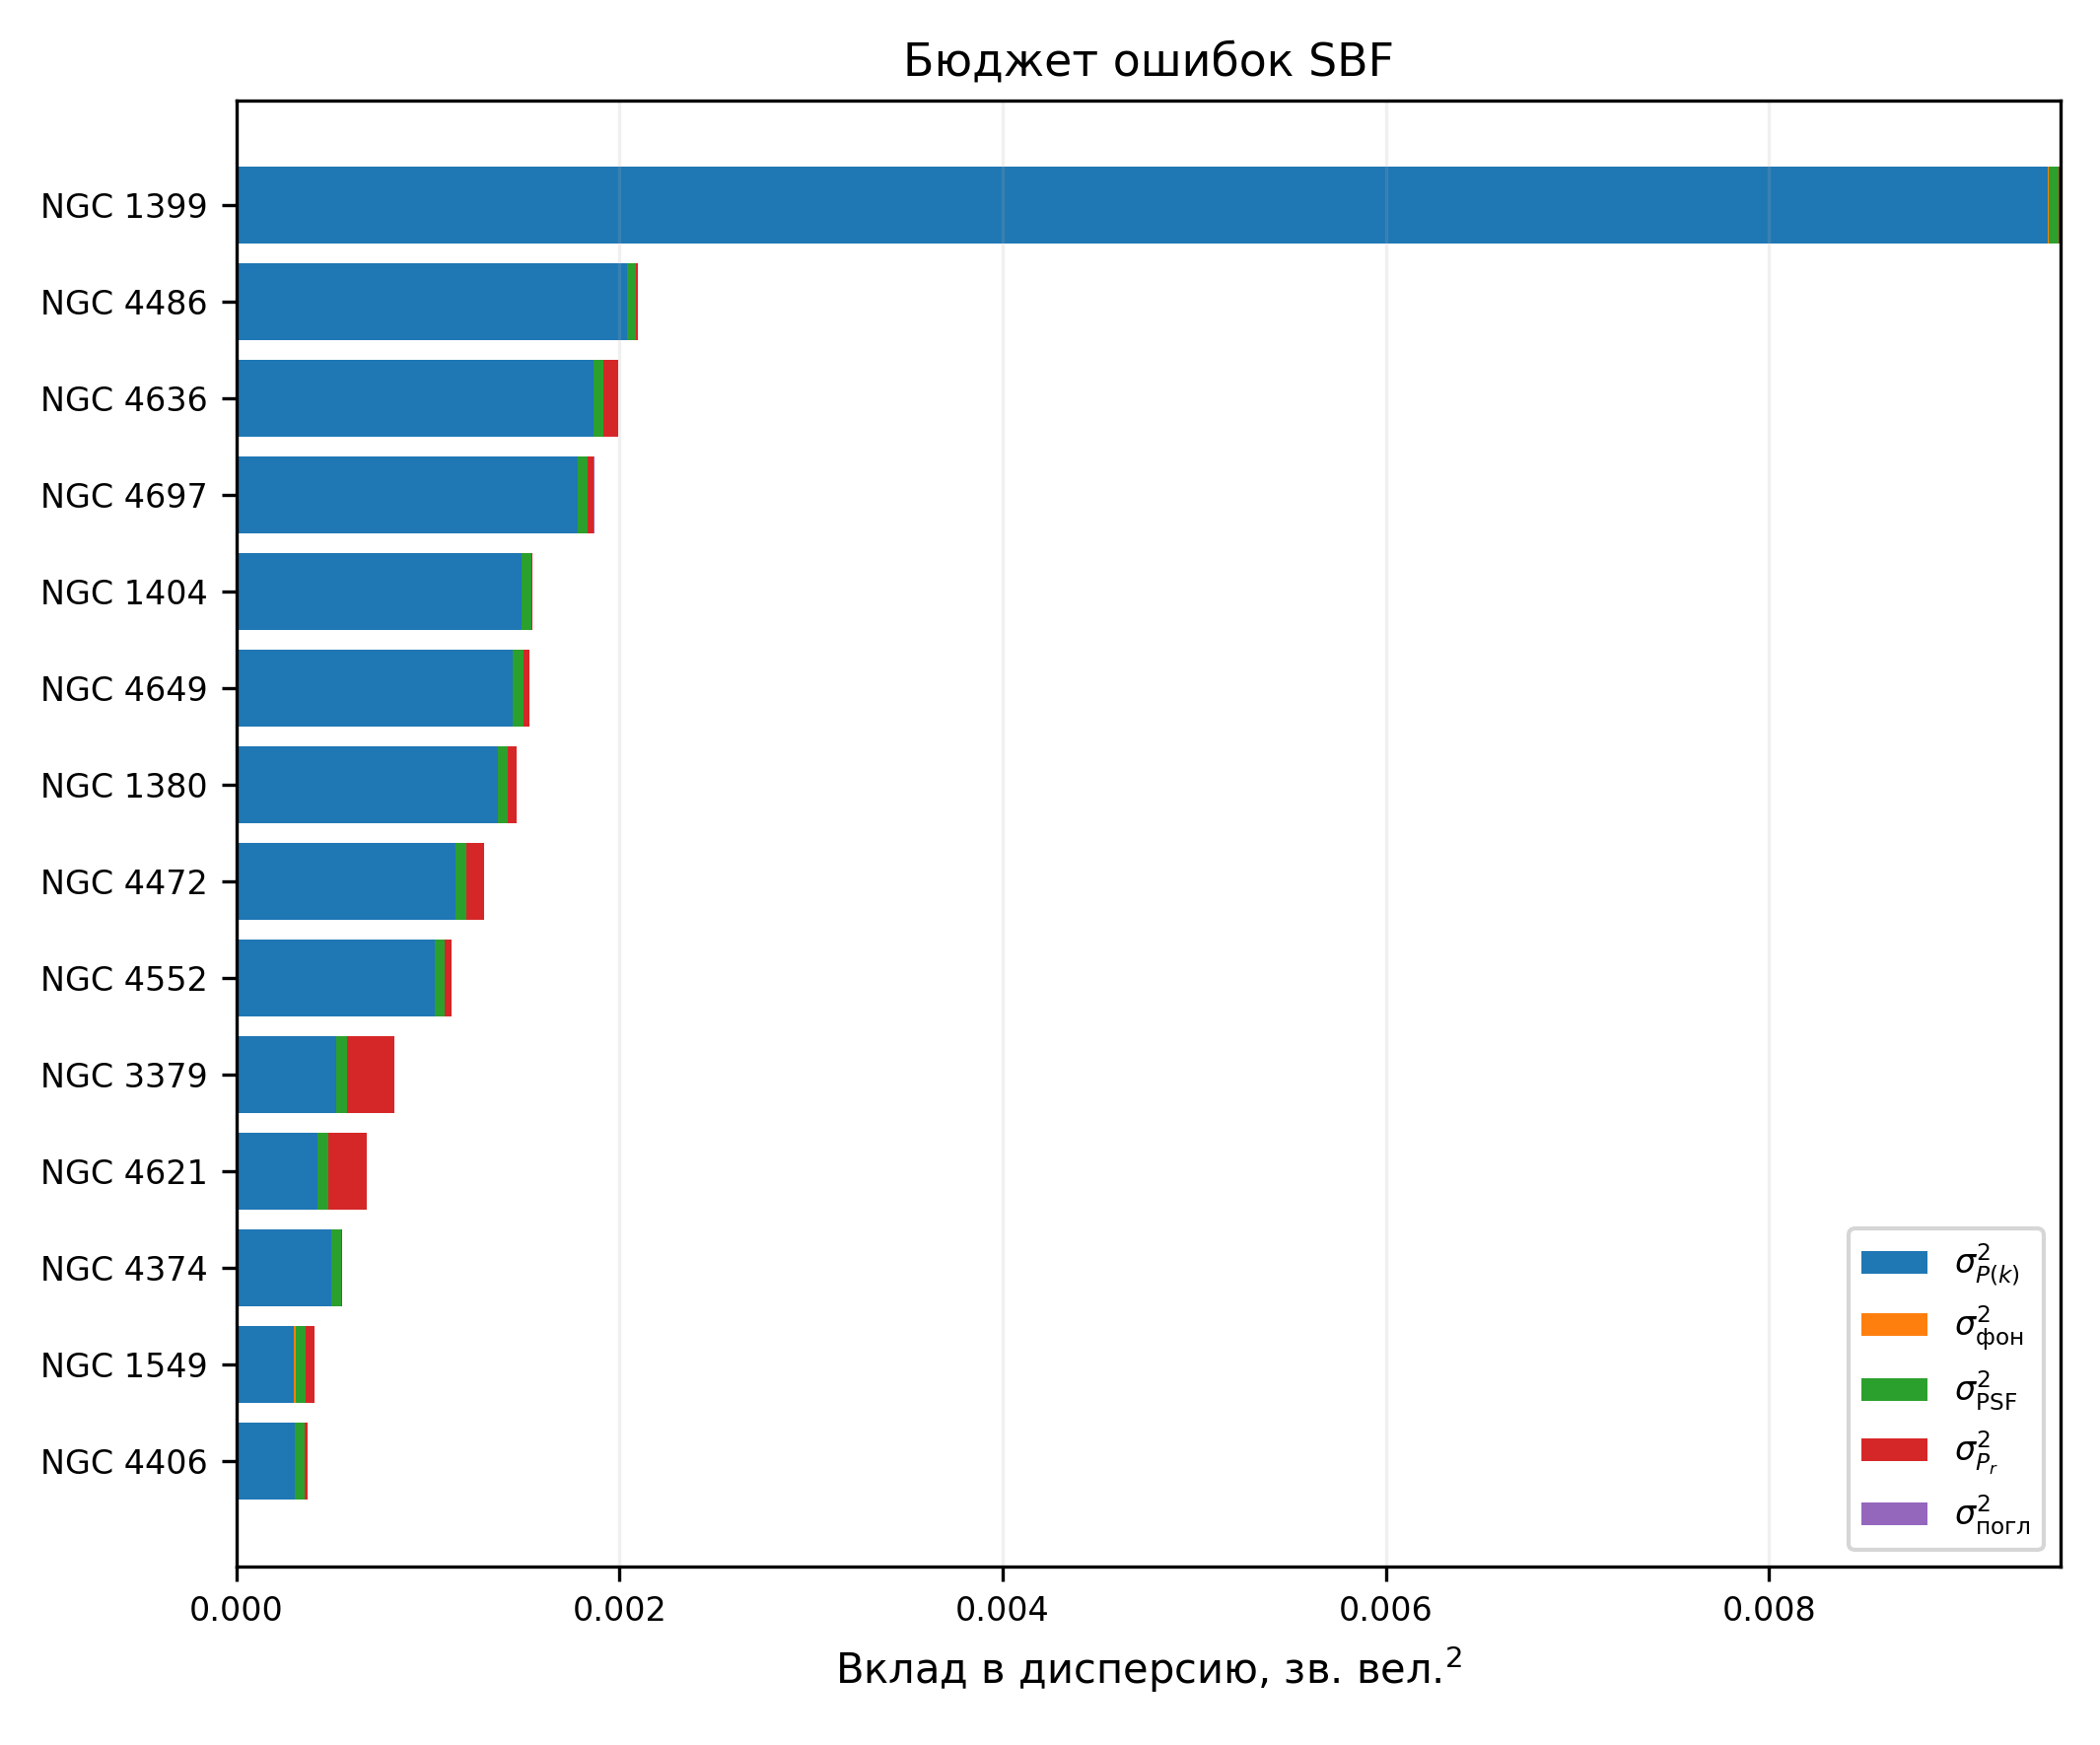
\includegraphics[width=0.94\textwidth]{BukanovIA/fig_errors.png}
    \caption{Вклады отдельных компонент в дисперсию ошибки $\overline m_{150}$. Цветами показаны слагаемые уравнения~(\ref{buk:eq:error_budget}).}
    \label{buk:fig:errors}
\end{figure}

\section{Калибровка по цвету}

Для каждой галактики абсолютная величина вычислялась по опорному TRGB-модулю расстояния:
\begin{equation}
    \overline M_{150}=\overline m_{150}-\mu_{\rm TRGB}.
\end{equation}
Цвет $C=F090W-F150W$ использовался как наблюдаемый индикатор звёздного населения. По 12 объектам основной выборки без существенных модельных предупреждений получена линейная калибровка
\begin{equation}
 \overline M_{150}=(-3.454\pm0.013)
 +(1.17\pm0.21)(C-0.40).
 \label{buk:eq:calibration}
\end{equation}
Внутренний разброс, необходимый для получения $\chi^2_{\rm red}\simeq1$, составил $\sigma_{\rm int}=0.049$ зв.~вел., а внутривыборочный взвешенный разброс остатков --- $0.059$ зв.~вел. Центрирование на $C=0.40$ не имеет отдельного физического смысла и только уменьшает ковариацию нуль-пункта и наклона.

\begin{figure}[H]
    \centering
    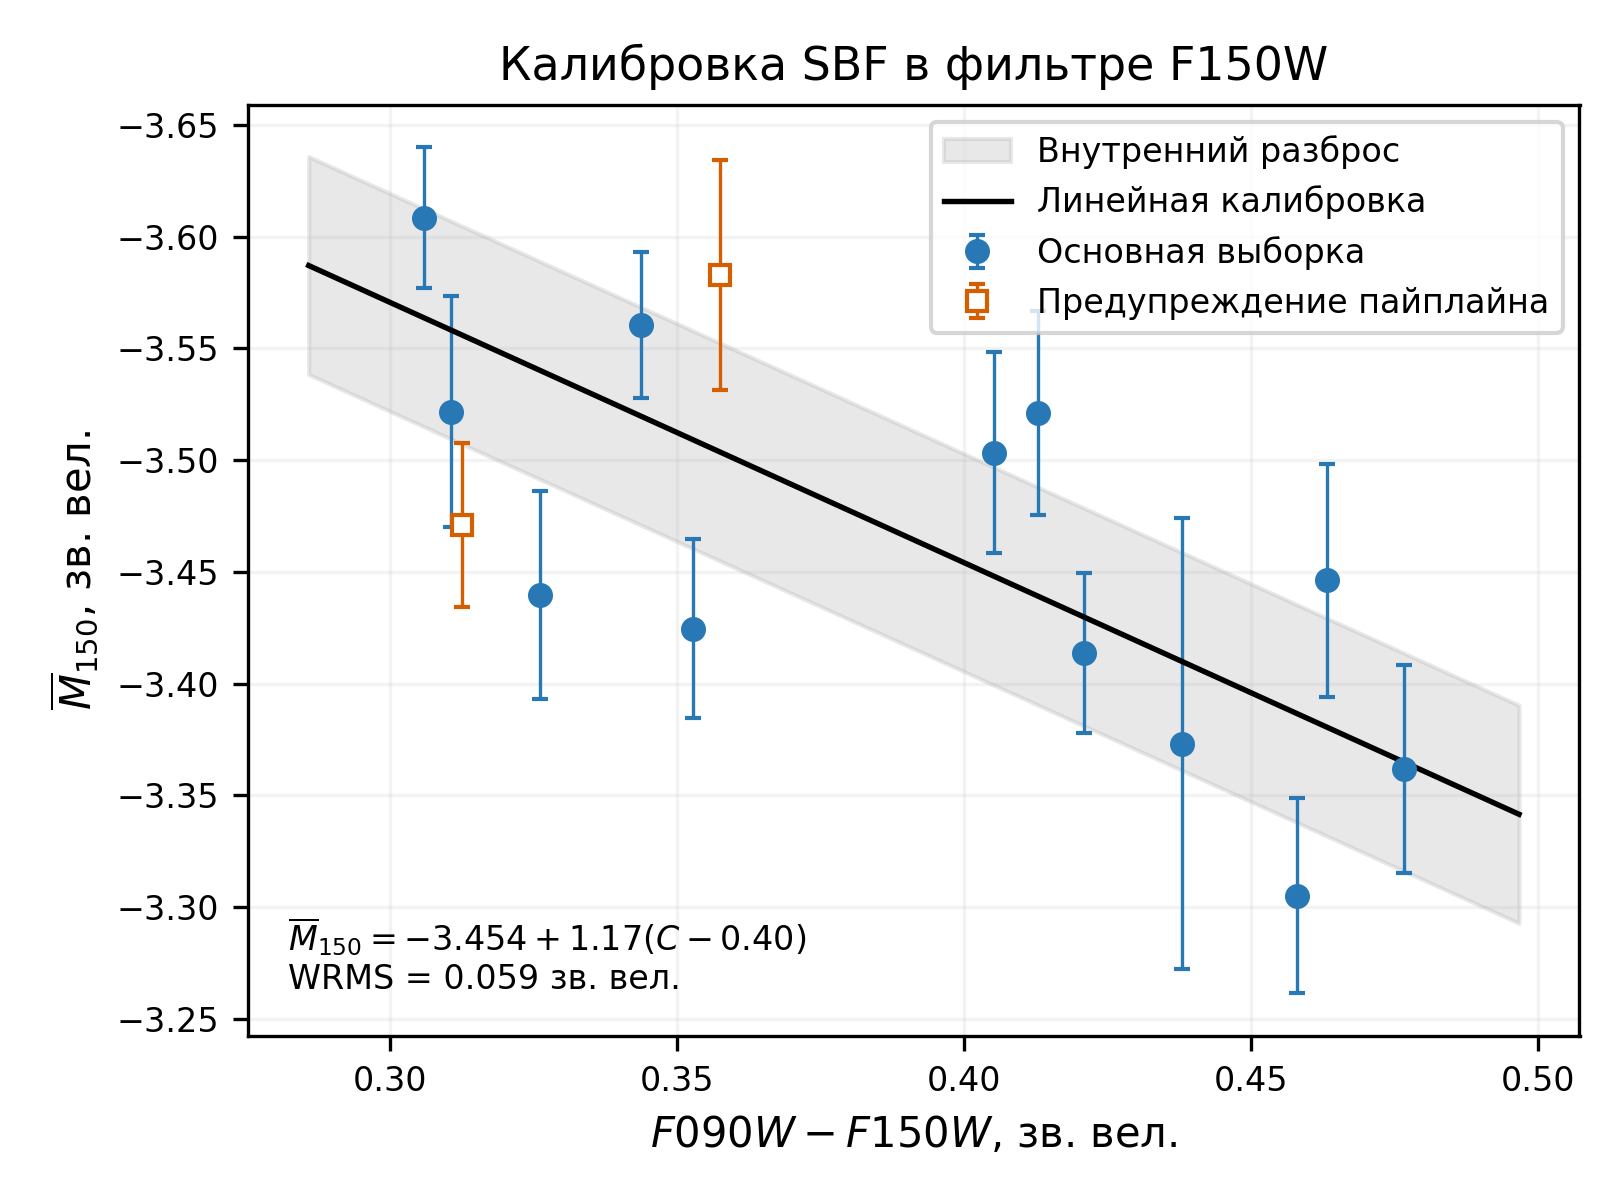
\includegraphics[width=0.83\textwidth]{BukanovIA/fig_calibration.png}
    \caption{Калибровка абсолютной флуктуационной величины в F150W по цвету. Синими точками показана основная выборка, оранжевыми квадратами --- объекты с предупреждениями пайплайна; серая область соответствует внутреннему разбросу.}
    \label{buk:fig:calibration}
\end{figure}

Постоянная, линейная и квадратичная модели сравнивались не только по исходным остаткам, но и методом последовательного исключения одного объекта (leave-one-out, LOO). Результаты приведены в табл.~\ref{buk:tab:models}. Линейная модель давала минимальный LOO-разброс; квадратичная зависимость почти не улучшала описание исходной выборки и хуже переносилась на исключённые объекты.

\begin{table}[ht]
\centering
\caption{Сравнение моделей цветовой калибровки.}
\label{buk:tab:models}
\small
\begin{tabular}{lcc}
\hline
Модель & WRMS выборки, зв. вел. & LOO WRMS, зв. вел.\\
\hline
Постоянная & 0.091 & 0.102\\
Линейная & 0.059 & 0.073\\
Квадратичная & 0.059 & 0.084\\
\hline
\end{tabular}
\end{table}

\section{Расстояния}

По уравнению~(\ref{buk:eq:calibration}) модуль расстояния определяется как
\begin{equation}
    \mu_{150}=\overline m_{150}-\overline M_{150}(C),
\end{equation}
а расстояние в мегапарсеках --- как $D=10^{(\mu-25)/5}$. Результаты для всех 14 галактик приведены в табл.~\ref{buk:tab:distances}. Ошибка $\mu_{150}$ включает измерительную ошибку $\overline m_{150}$ и $\sigma_{\rm int}$, но не общую систематику нуль-пункта TRGB.

\begin{table}[H]
\centering
\caption{Измеренные SBF-величины и восстановленные модули расстояния. Звёздочкой отмечены объекты, не использованные в основном фите.}
\label{buk:tab:distances}
\scriptsize
\setlength{\tabcolsep}{3.2pt}
\begin{tabular}{lcccc}
\hline
Галактика & $F090W-F150W$ & $\overline m_{150}$ & $\mu_{150}$ & $\mu_{\rm TRGB}$\\
\hline
NGC~1380 & 0.413 & $27.887\pm0.038$ & $31.326\pm0.062$ & $31.408\pm0.025$\\
NGC~1399 & 0.438 & $28.125\pm0.098$ & $31.535\pm0.109$ & $31.498\pm0.026$\\
NGC~1404 & 0.477 & $28.004\pm0.039$ & $31.369\pm0.063$ & $31.366\pm0.025$\\
NGC~1549 & 0.344 & $27.670\pm0.020$ & $31.190\pm0.053$ & $31.231\pm0.026$\\
NGC~3379 & 0.353 & $26.654\pm0.029$ & $30.163\pm0.057$ & $30.078\pm0.028$\\
NGC~4374 & 0.421 & $27.698\pm0.024$ & $31.128\pm0.054$ & $31.112\pm0.027$\\
NGC~4406 & 0.306 & $27.487\pm0.019$ & $31.051\pm0.052$ & $31.096\pm0.025$\\
NGC~4472 & 0.405 & $27.513\pm0.036$ & $30.961\pm0.061$ & $31.016\pm0.027$\\
NGC~4486 & 0.463 & $27.600\pm0.046$ & $30.980\pm0.067$ & $31.046\pm0.025$\\
NGC~4552 & 0.458 & $27.618\pm0.034$ & $31.005\pm0.059$ & $30.923\pm0.028$\\
NGC~4621$^{*}$ & 0.313 & $27.350\pm0.026$ & $30.906\pm0.055$ & $30.821\pm0.026$\\
NGC~4636 & 0.311 & $27.548\pm0.045$ & $31.107\pm0.066$ & $31.070\pm0.026$\\
NGC~4649 & 0.326 & $27.569\pm0.039$ & $31.110\pm0.063$ & $31.009\pm0.025$\\
NGC~4697$^{*}$ & 0.358 & $26.741\pm0.043$ & $30.245\pm0.065$ & $30.324\pm0.028$\\
\hline
\end{tabular}
\end{table}

Для основной выборки среднее взвешенное отличие от опорной шкалы равно
\begin{equation}
 \left\langle\mu_{150}-\mu_{\rm TRGB}\right\rangle
 =0.003\pm0.019\ {\rm mag},
\end{equation}
а WRMS остатков составляет $0.061$ зв.~вел. (рис.~\ref{buk:fig:distances}). Поскольку те же объекты участвовали в калибровке, это сравнение характеризует внутреннее согласие, а не полностью независимую проверку.

\begin{figure}[H]
    \centering
    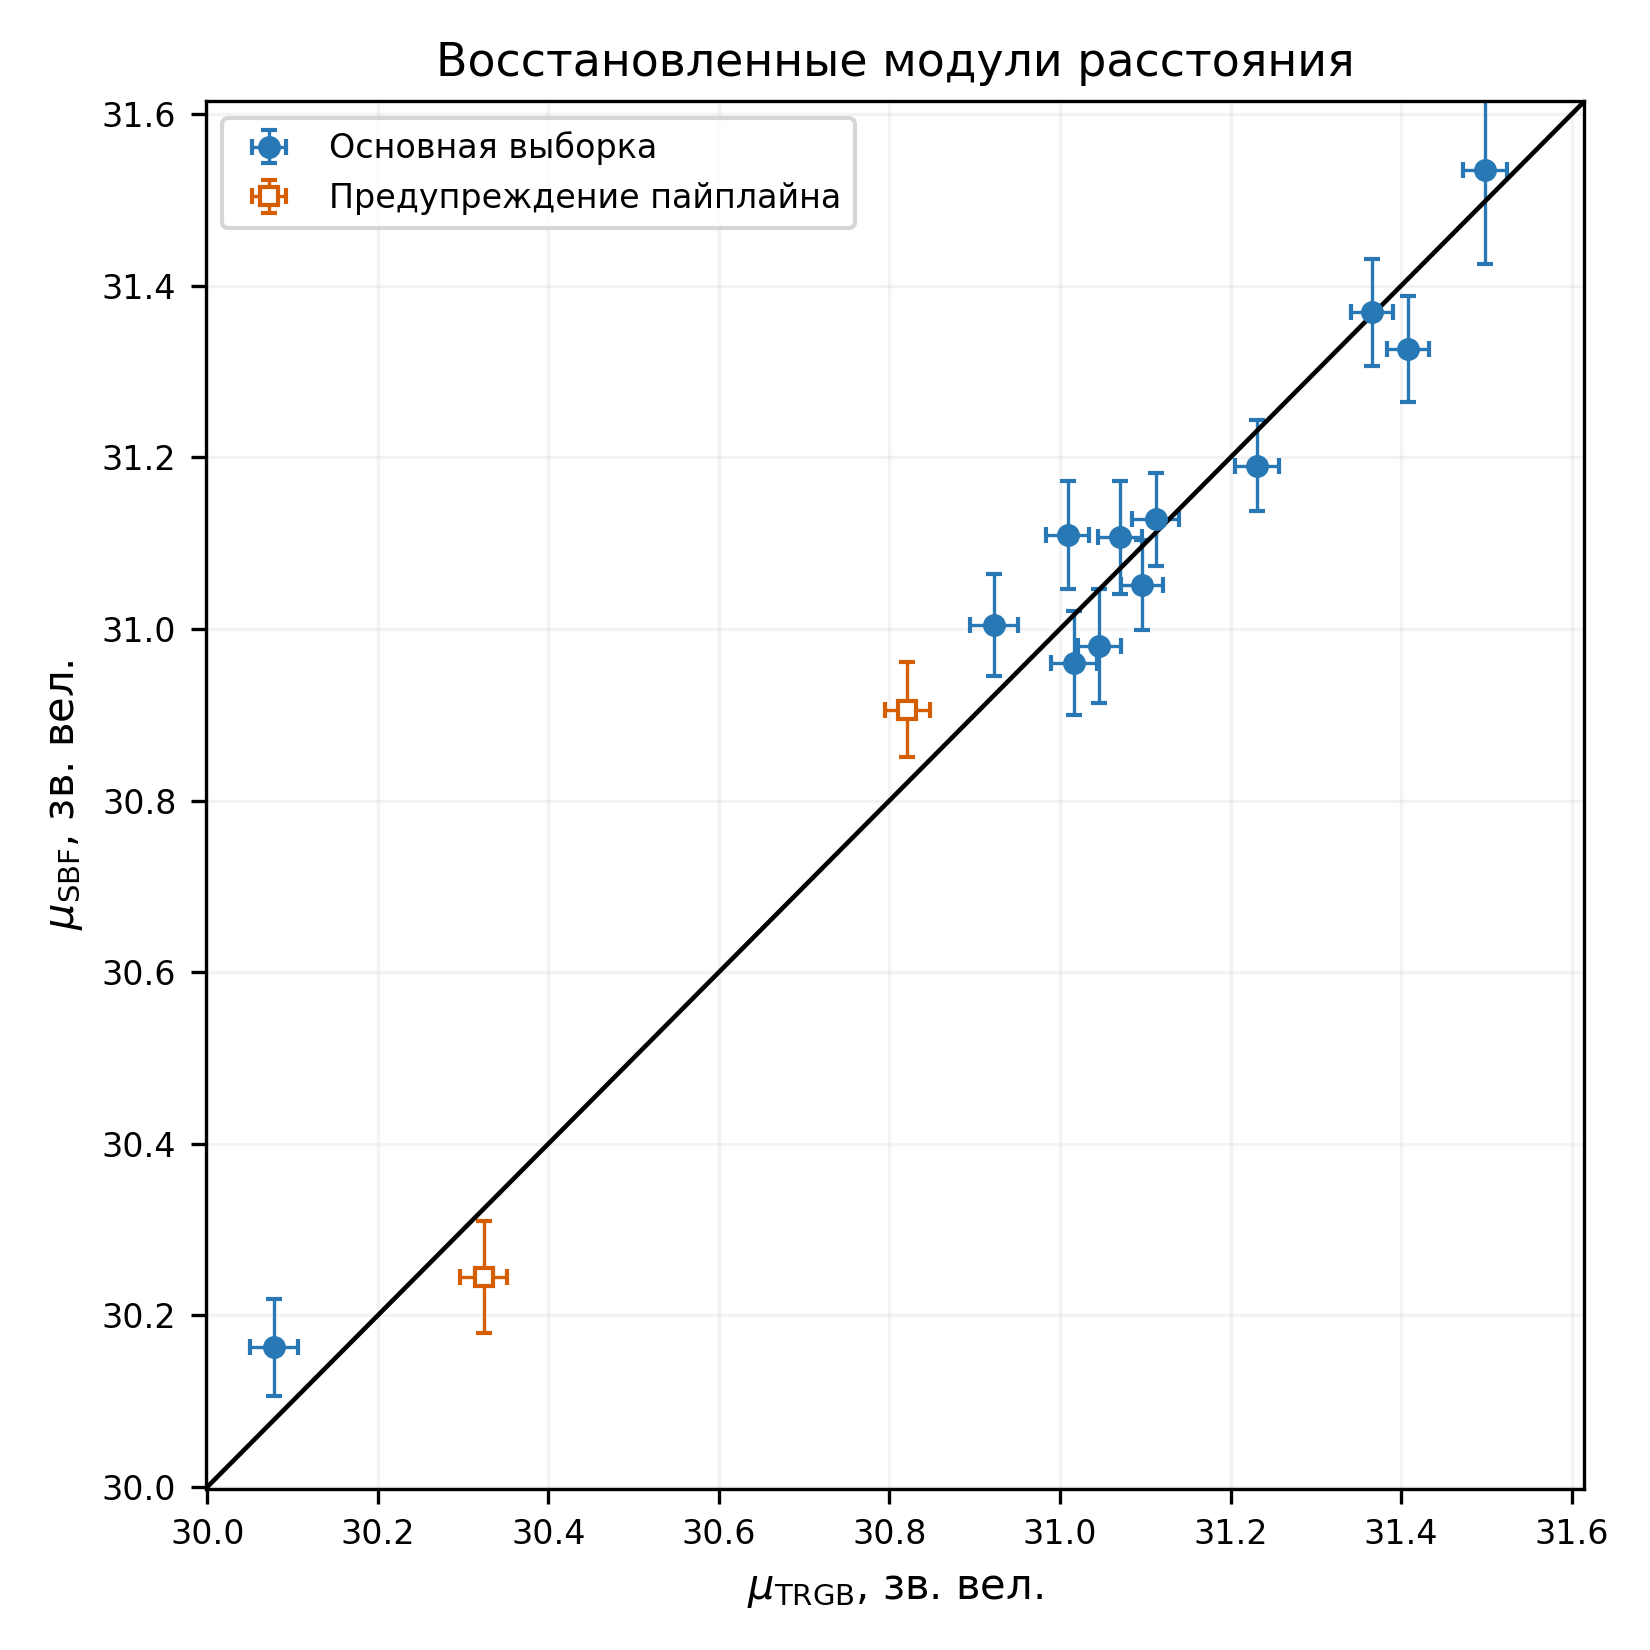
\includegraphics[width=0.70\textwidth]{BukanovIA/fig_distances.png}
    \caption{Сравнение модулей расстояния, восстановленных по F150W SBF, с индивидуальными TRGB-модулями. Диагональ соответствует равенству оценок.}
    \label{buk:fig:distances}
\end{figure}

В LOO-тесте каждая галактика по очереди исключалась, калибровка строилась по остальным объектам, после чего восстанавливалось расстояние до исключённой галактики. Полученный WRMS равен $0.073$ зв.~вел. Относительная ошибка расстояния связана с ошибкой модуля соотношением $\Delta D/D\simeq(\ln10/5)\Delta\mu$; следовательно, $0.073$ зв.~вел. соответствует приблизительно $3.4\%$. Для постоянной калибровки LOO-разброс равен $0.102$ зв.~вел., или $4.7\%$.

\subsection{Сравнение с HST/F160W}

Для пяти галактик имеются опубликованные измерения HST/WFC3 в фильтре F160W~\cite{Jensen2015}. Среднее взвешенное различие составляет
\begin{equation}
 \left\langle\mu_{150}-\mu_{160,\rm Jensen}\right\rangle
 =-0.063\pm0.067\ {\rm mag},
\end{equation}
при WRMS $0.105$ зв.~вел. (рис.~\ref{buk:fig:jensen}). Найденное смещение статистически согласуется с нулём и по порядку величины соответствует известному различию TRGB- и более ранней Cepheid/SBF-шкал~\cite{Jensen2025}.

\begin{figure}[H]
    \centering
    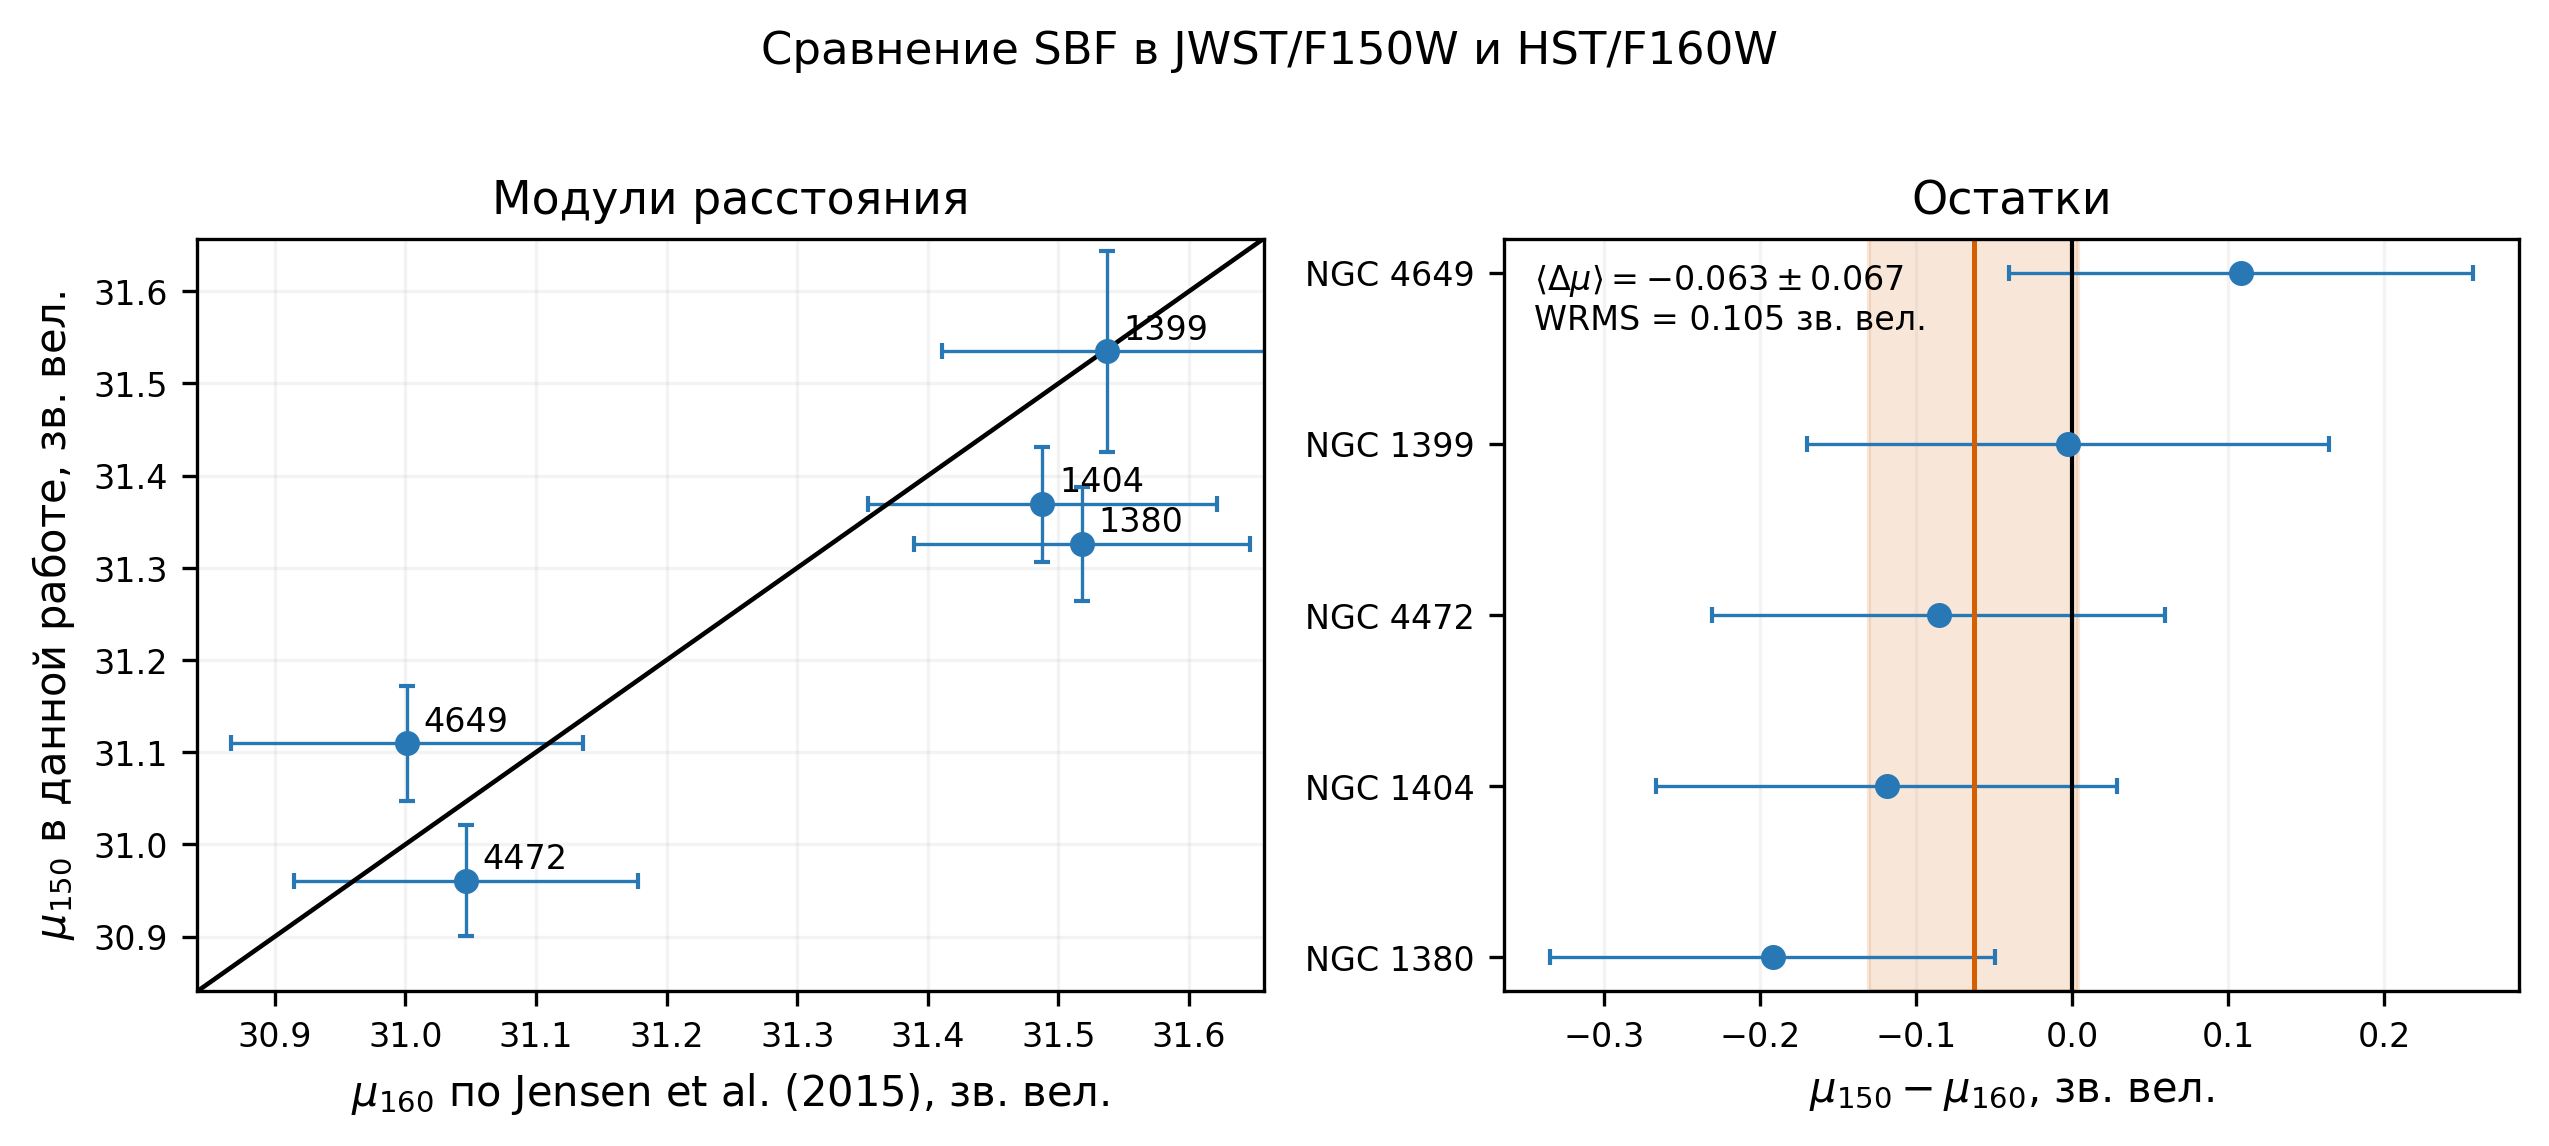
\includegraphics[width=0.96\textwidth]{BukanovIA/fig_jensen.png}
    \caption{Сравнение модулей расстояния по JWST/F150W и опубликованной калибровке HST/F160W для пяти общих галактик.}
    \label{buk:fig:jensen}
\end{figure}

\section{Обсуждение}

В рамках выполненного анализа линейный цветовой член уменьшает LOO-разброс относительно постоянной калибровки. Такой результат физически ожидаем, поскольку SBF сильнее обычной интегральной фотометрии зависит от наиболее ярких звёзд, а цвет частично характеризует возраст и металличность населения. Однако выборка мала, цветовой диапазон узок, а две галактики имеют предупреждения моделирования. Поэтому полученный наклон следует рассматривать как первую эмпирическую калибровку F150W, а не как окончательный закон для всех типов галактик.

К главным систематическим ограничениям относятся качество гладкой модели, маскирование компактных источников, описание PSF и оценка $P_r$. Крупномасштабные остатки модели способны попадать в низкочастотную часть $P(k)$, а незамаскированные источники увеличивают его амплитуду. Использование двух колец, проверки вариантов сэмплирования PSF и ограниченного частотного диапазона снижает чувствительность к этим эффектам, но не устраняет её полностью. Дальнейшая проверка требует независимой выборки галактик и единого анализа более широкого диапазона цветов.

\section{Заключение}

По изображениям \textit{JWST}/NIRCam измерены F150W SBF-величины 14 ранних галактик программы GO-3055. Построена изофотная модель каждого объекта, учтены маска, PSF и вклад неразрешённых источников. По 12 основным объектам получена линейная цветовая калибровка с внутренним разбросом $0.049$ зв.~вел. LOO-разброс восстановленных модулей расстояния составил $0.073$ зв.~вел., или около $3.4\%$ по расстоянию. Среднее отличие от индивидуальной TRGB-шкалы равно $0.003\pm0.019$ зв.~вел.; сравнение пяти общих объектов с HST/F160W не выявило значимого смещения. Результат показывает применимость JWST/F150W SBF к измерению расстояний и одновременно подчёркивает необходимость расширения независимой калибровочной выборки.

\begin{thebibliography}{99}

\bibitem{TonrySchneider1988}
Tonry~J.~L., Schneider~D.~P. A new technique for measuring extragalactic distances // The Astronomical Journal. --- 1988. --- Vol.~96, no.~3. --- P.~807--815. DOI: 10.1086/114847.

\bibitem{Jensen2015}
Jensen~J.~B., Blakeslee~J.~P., Gibson~Z., Lee~H.-c., Cantiello~M., Raimondo~G., Boyer~N., Cho~H. Measuring infrared surface brightness fluctuation distances with HST WFC3: calibration and advice // The Astrophysical Journal. --- 2015. --- Vol.~808, no.~1. --- Art.~91. DOI: 10.1088/0004-637X/808/1/91.

\bibitem{Blakeslee2021}
Blakeslee~J.~P., Jensen~J.~B., Ma~C.-P., Milne~P.~A., Greene~J.~E. The Hubble Constant from infrared surface brightness fluctuation distances // The Astrophysical Journal. --- 2021. --- Vol.~911, no.~1. --- Art.~65. DOI: 10.3847/1538-4357/abe86a.

\bibitem{Anand2024}
Anand~G.~S., Tully~R.~B., Cohen~Y., Makarov~D.~I., Makarova~L.~N., Jensen~J.~B., Blakeslee~J.~P., Cantiello~M., Kourkchi~E., Raimondo~G. The Population II Extragalactic Distance Scale: A TRGB Distance to the Fornax Cluster with JWST // The Astrophysical Journal. --- 2024. --- Vol.~973, no.~2. --- Art.~83. DOI: 10.3847/1538-4357/ad64c7.

\bibitem{Jensen2025}
Jensen~J.~B., Blakeslee~J.~P., Cantiello~M., Cowles~M., Anand~G.~S., Tully~R.~B., Kourkchi~E., Raimondo~G. The TRGB--SBF Project. III. Refining the HST surface brightness fluctuation distance scale calibration with JWST // The Astrophysical Journal. --- 2025. --- Vol.~987, no.~1. --- Art.~87. DOI: 10.3847/1538-4357/addfd6.

\bibitem{Chazov2026}
Chazov~M.~I., Makarov~D.~I., Tully~R.~B., Anand~G.~S., Makarova~L.~N., Cohen~Y., Blakeslee~J.~P., Cantiello~M., Jensen~J.~B., Raimondo~G. The TRGB--SBF Project. IV. A color calibration of the TRGB in the JWST F090W+F150W filters [Электронный ресурс] // arXiv. --- 2026. --- arXiv:2603.11160. DOI: 10.48550/arXiv.2603.11160. --- URL: \url{https://arxiv.org/abs/2603.11160} (дата обращения: 22.08.2026).

\bibitem{MAST}
Barbara A. Mikulski Archive for Space Telescopes (MAST) [Электронный ресурс] / Space Telescope Science Institute. --- URL: \url{https://mast.stsci.edu} (дата обращения: 22.08.2026).

\bibitem{GitHubRepo}
Bukanov~I.~A. Код, таблицы и графики проекта по методу SBF [Электронный ресурс] // GitHub. --- URL: \url{https://github.com/Saharochekl/course-work_4-SBF} (дата обращения: 22.08.2026).

\bibitem{Richard2024Siril}
Richard~C., Hourdin~V., M\'elis~C., Knagg-Baugh~A. Siril: An Advanced Tool for Astronomical Image Processing // Journal of Open Source Software. --- 2024. --- Vol.~9, no.~102. --- Art.~7242. DOI: 10.21105/joss.07242.

\end{thebibliography}
